%%%%%%%%%%%%%%%%%%%%%%%%%%%%%%%%%%%%%%%%%
% Beamer Presentation
% LaTeX Template
% Version 1.0 (10/11/12)
%
% This template has been downloaded from:
% http://www.LaTeXTemplates.com
%
% License:
% CC BY-NC-SA 3.0 (http://creativecommons.org/licenses/by-nc-sa/3.0/)
%
%%%%%%%%%%%%%%%%%%%%%%%%%%%%%%%%%%%%%%%%%

%----------------------------------------------------------------------------------------
%	PACKAGES AND THEMES
%----------------------------------------------------------------------------------------

\documentclass{beamer}

\mode<presentation> {

% The Beamer class comes with a number of default slide themes
% which change the colors and layouts of slides. Below this is a list
% of all the themes, uncomment each in turn to see what they look like.

%\usetheme{default}
%\usetheme{AnnArbor}
%\usetheme{Antibes}
%\usetheme{Bergen}
%\usetheme{Berkeley}
%\usetheme{Berlin}
%\usetheme{Boadilla}
%\usetheme{CambridgeUS}
%\usetheme{Copenhagen}
%\usetheme{Darmstadt}
%\usetheme{Dresden}
%\usetheme{Frankfurt}
%\usetheme{Goettingen}
%\usetheme{Hannover}
%\usetheme{Ilmenau}
%\usetheme{JuanLesPins}
%\usetheme{Luebeck}
\usetheme{Madrid}
%\usetheme{Malmoe}
%\usetheme{Marburg}
%\usetheme{Montpellier}
%\usetheme{PaloAlto}
%\usetheme{Pittsburgh}
%\usetheme{Rochester}
%\usetheme{Singapore}
%\usetheme{Szeged}
%\usetheme{Warsaw}

% As well as themes, the Beamer class has a number of color themes
% for any slide theme. Uncomment each of these in turn to see how it
% changes the colors of your current slide theme.

%\usecolortheme{albatross}
%\usecolortheme{beaver}
%\usecolortheme{beetle}
%\usecolortheme{crane}
%\usecolortheme{dolphin}
%\usecolortheme{dove}
%\usecolortheme{fly}
%\usecolortheme{lily}
%\usecolortheme{orchid}
%\usecolortheme{rose}
%\usecolortheme{seagull}
%\usecolortheme{seahorse}
%\usecolortheme{whale}
%\usecolortheme{wolverine}

%\setbeamertemplate{footline} % To remove the footer line in all slides uncomment this line
%\setbeamertemplate{footline}[page number] % To replace the footer line in all slides with a simple slide count uncomment this line

%\setbeamertemplate{navigation symbols}{} % To remove the navigation symbols from the bottom of all slides uncomment this line
}

\usepackage{graphicx} % Allows including images
\usepackage{booktabs} % Allows the use of \toprule, \midrule and \bottomrule in tables

%----------------------------------------------------------------------------------------
%	TITLE PAGE
%----------------------------------------------------------------------------------------

\title[Market simulator]{FiQuant Market Microstructure Simulator} % The short title appears at the bottom of every slide, the full title is only on the title page

\author{Anton Kolotaev} % Your name
\institute[ECP] % Your institution as it will appear on the bottom of every slide, may be shorthand to save space
{
Ecole Centrale de Paris \\ % Your institution for the title page
\medskip
\textit{anton.kolotaev@gmail.com} % Your email address
}
\date{\today} % Date, can be changed to a custom date

\begin{document}

\begin{frame}
\titlepage % Print the title page as the first slide
\end{frame}

\begin{frame}
\frametitle{Overview} % Table of contents slide, comment this block out to remove it
\tableofcontents % Throughout your presentation, if you choose to use \section{} and \subsection{} commands, these will automatically be printed on this slide as an overview of your presentation
\end{frame}

%----------------------------------------------------------------------------------------
%	PRESENTATION SLIDES
%----------------------------------------------------------------------------------------

%------------------------------------------------
\section{Installation} % Sections can be created in order to organize your presentation into discrete blocks, all sections and subsections are automatically printed in the table of contents as an overview of the talk
%------------------------------------------------
\begin{frame}
\frametitle{Requirements}
\begin{itemize}
\item OS supported: Linux, Mac OS X, Windows
\item Browsers supported: Chrome, Firefox, Safari, Opera
\item Python 2.7
\item Python packages can be installed using \texttt{pip} or \texttt{easyinstall}:
\begin{itemize}
\item \href{http://home.gna.org/veusz/}{Veusz} (for graph plotting)
\item \href{http://flask.pocoo.org}{Flask} (to run a Web-server)
\item \href{https://pypi.python.org/pypi/blist/}{Blist} (sorted collections used by ArbitrageTrader) 
\end{itemize}
\item Source code downloadable from \href{http://sourceforge.net/p/marketsimulator/svn/HEAD/tree/DevAnton/v3/}{SourceForge}
\end{itemize}

\end{frame}

\section{Simulator components}
\subsection{Scheduler} % A subsection can be created just before a set of slides with a common theme to further break down your presentation into chunks
\begin{frame}
\frametitle{Scheduler}
\begin{itemize}
  \item Main class for every discrete event simulation system.
  \item Maintains a set of actions to fulfill in future and launches them according their action times: from older ones to newer.
\end{itemize}
Interface:
\begin{itemize}
  \item Event scheduling:
  \begin{itemize}
    \item \texttt{schedule(actionTime, handler)}
    \item \texttt{scheduleAfter(dt, handler)}
  \end{itemize}
  \item Simulation control:
  \begin{itemize}
    \item \texttt{workTill(limitTime)}
    \item \texttt{advance(dt)}
    \item \texttt{reset()}
  \end{itemize}
\end{itemize}
\end{frame}

%------------------------------------------------
\subsection{Order books} % A subsection can be created just before a set of slides with a common theme to further break down your presentation into chunks
\begin{frame}
\frametitle{Order book}
\begin{itemize}
  \item Represents a single asset traded in some market (Same asset traded in different markets would be represented by different order books)
  \item Matches incoming orders
  \item Stores unfulfilled limit orders in two order queues (\texttt{Asks} for sell orders and \texttt{Bids} for buy orders)
  \item Corrects limit order price with respect to tick size
  \item Imposes order processing fee
  \item Supports queries about order book structure
  \item Notifies listeners about trades and price changes
\end{itemize}
\end{frame}

%------------------------------------------------
\begin{frame}
\frametitle{Order book for a remote trader}
\begin{itemize}
  \item Models a trader connected to a market by a communication channel with non-negligible latency
  \item Introduces delay in information propagation from a trader to an order book and vice versa (so a trader has outdated information about market and orders are sent to the market with a certain delay)
  \item Assures correct order of messages: older messages always come earlier than newer ones
\end{itemize}
\end{frame}

%------------------------------------------------
\subsection{Orders} 
\begin{frame}
\frametitle{Basic orders}
Orders supported internally by an order book:
\begin{itemize}
  \item \texttt{Market(side, volume)}
  \item \texttt{Limit(side, price, volume)}
  \item \texttt{Cancel(limitOrder)}
\end{itemize}
Limit and market orders notifies their listeners about all trades they take part in.
Factory functions are usually used in order to create orders.
\end{frame}

%------------------------------------------------
\begin{frame}
\frametitle{Meta orders}
Follow order interface from trader's perspective (so they can be used instead of basic orders) but behave like a sequence of base orders from an order book point of view.
\begin{itemize}
  \item \texttt{Iceberg(volumeLimit, orderToSplit)} splits \texttt{orderToSplit} to pieces with volume less than \texttt{volumeLimit} and sends them one by one to an order book ensuring that only one order at time is processed there
  \item \texttt{AlwaysBest(volume, limitOrderFactory)} creates a limit-like order with given volume and the most attractive price, sends it to an order book and if the order book best price changes, cancels it and resends with a better price
  \item \texttt{WithExpiry(lifetime, limitOrderFactory)} sends a limit-like order and after \texttt{lifetime} cancels it
  \item \texttt{LimitMarket(limitOrderFactory)} is like \texttt{WithExpiry} but with \texttt{lifetime} equal to 0 
\end{itemize}
\end{frame}

%------------------------------------------------
\subsection{Traders}
\begin{frame}
\frametitle{Traders}
Single asset traders
\begin{itemize}
  \item send orders to order books
  \item bookkeep their position and balance
  \item run a number of trading strategies
  \item notify listeners about trades done and orders sent
\end{itemize}
Single asset traders operate on a single or multiple markets.
If a trader holds a portfolio composed of multiple assets it should aggregate an array of single asset traders.
\end{frame}

%------------------------------------------------
\subsection{Strategies}
\begin{frame}[fragile]
\frametitle{Generic strategy}
\begin{verbatim}
class Generic(Strategy):
  def __init__(self, eventGen, sideFunc, ...):
    # ... storing constructor arguments
    event.subscribe(self.eventGen, self.wakeUp)

  def wakeUp(self):
    if not self.suspended:
      # determine side and parameters of an order to create
      side = self.sideFunc()
      if side <> None:
        volume = int(self.volumeFunc())
        if volume > 0:
          # create order given side and parameters
          order = self.orderFactory(side)(volume)
          # send order to the order book
          self.trader.send(order)
\end{verbatim}
\end{frame}

%------------------------------------------------

\begin{frame}
\frametitle{Signal strategy}
Signal strategy listens to some discrete signal and when the signal becomes more than some threshold it starts to buy. When the signal gets lower than -threshold the strategy starts to sell.
\begin{figure}[htbp]
\centering
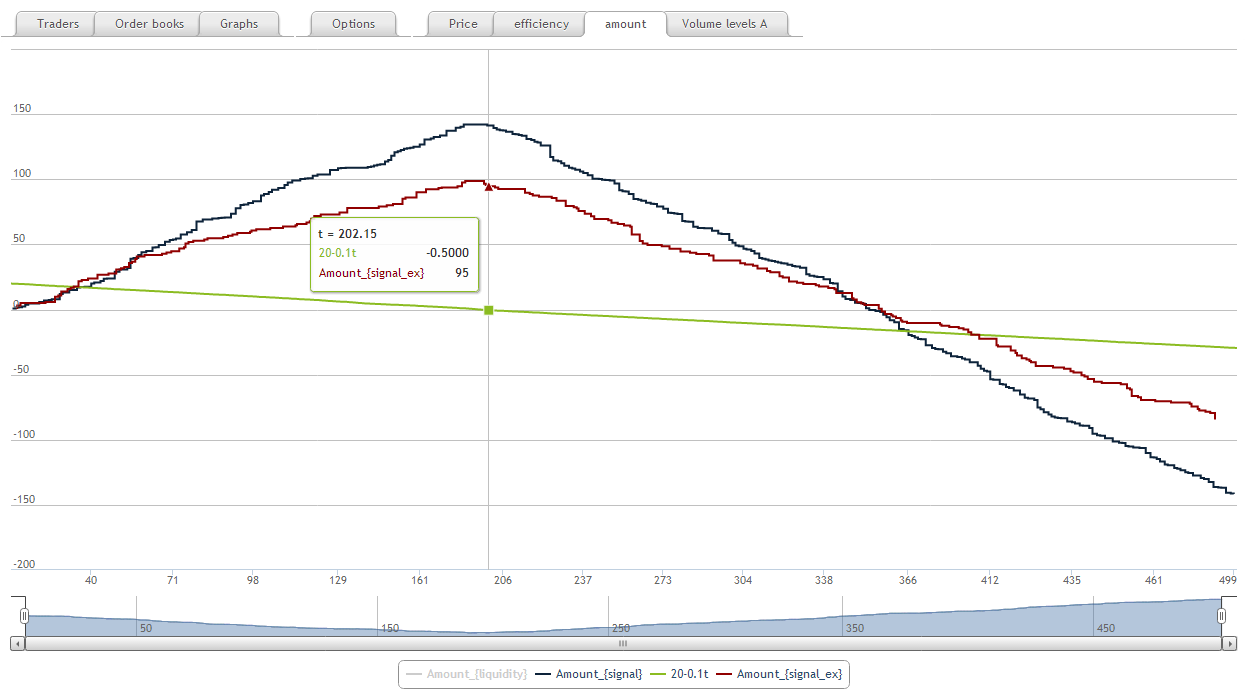
\includegraphics[width=1\linewidth]{signal.png}
\caption{Signal trader sample run (signal=20-t/10)}
\end{figure}
\end{frame}

%------------------------------------------------

\begin{frame}
\frametitle{Trend follower strategy}
Trend follower is an instance of a signal strategy with signal equal to the first derivative of a moving average of the asset's price (i.e trend).
\begin{figure}[htbp]
\centering
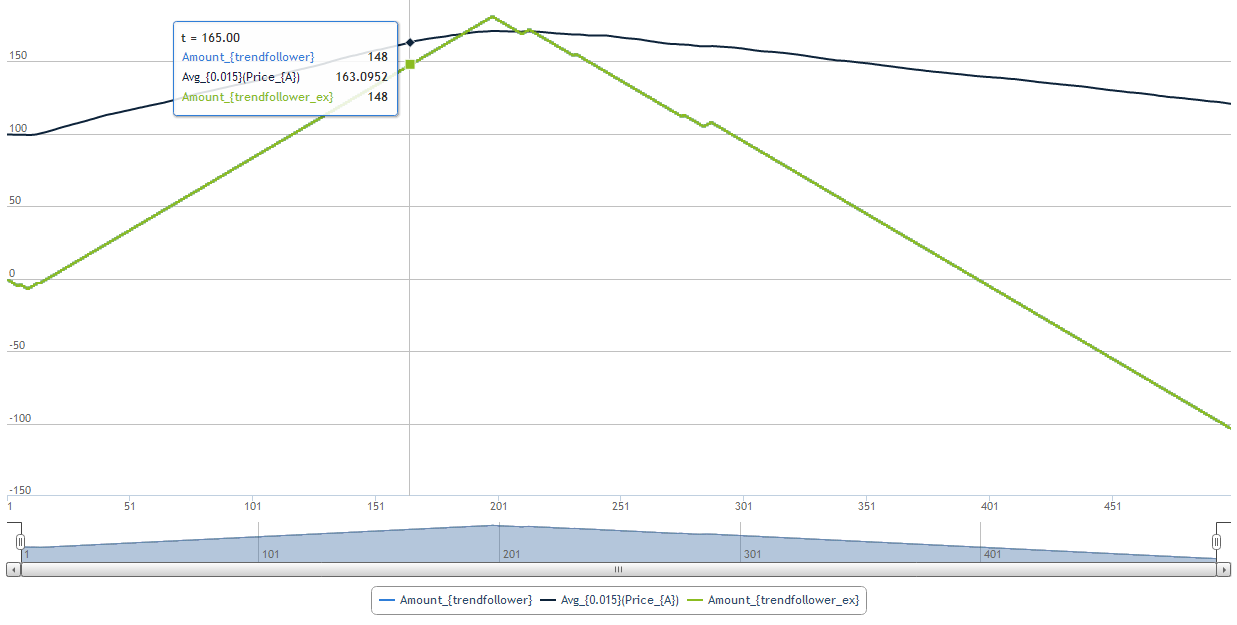
\includegraphics[width=1\linewidth]{trendfollower.png}
\end{figure}
\end{frame}

%------------------------------------------------

\begin{frame}
\frametitle{Two averages strategy}
Two averages is an instance of a signal strategy with signal equal to the difference between two moving averages of the asset's price (i.e trend).
\begin{figure}[htbp]
\centering
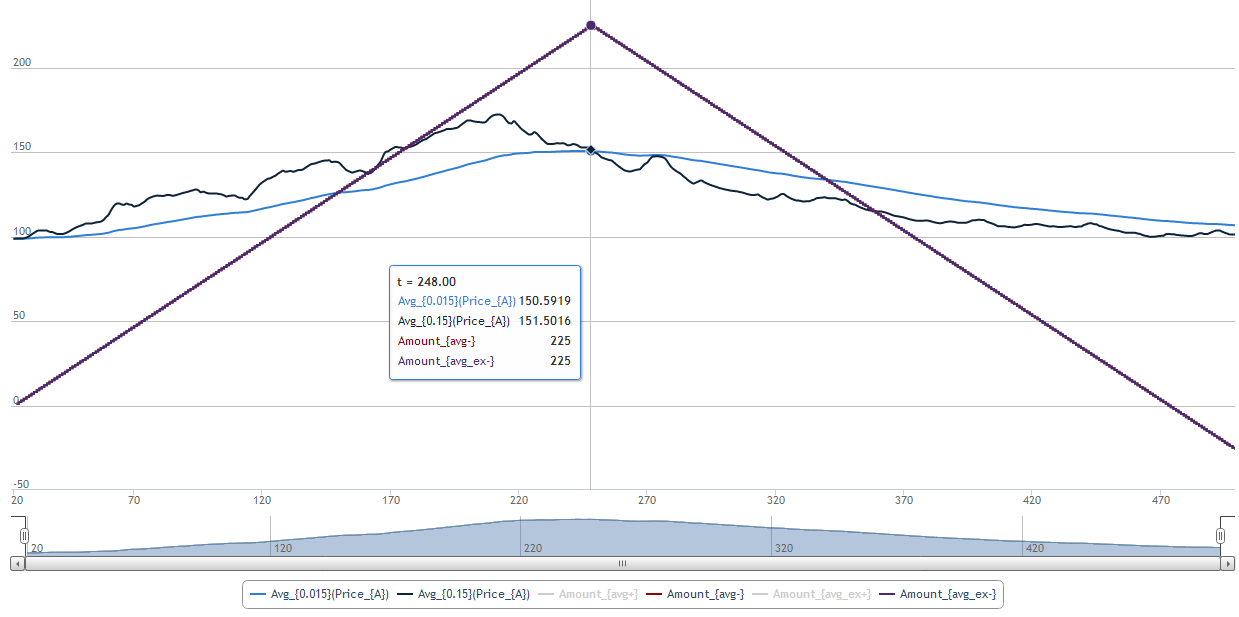
\includegraphics[width=1\linewidth]{twoaverages.png}
\end{figure}
\end{frame}
%------------------------------------------------

\begin{frame}
\frametitle{Fundamental value strategy}
Fundamental value strategy is an instance of a signal strategy with signal equal to the difference between the asset's price and some fundamental value.
\begin{figure}[htbp]
\centering
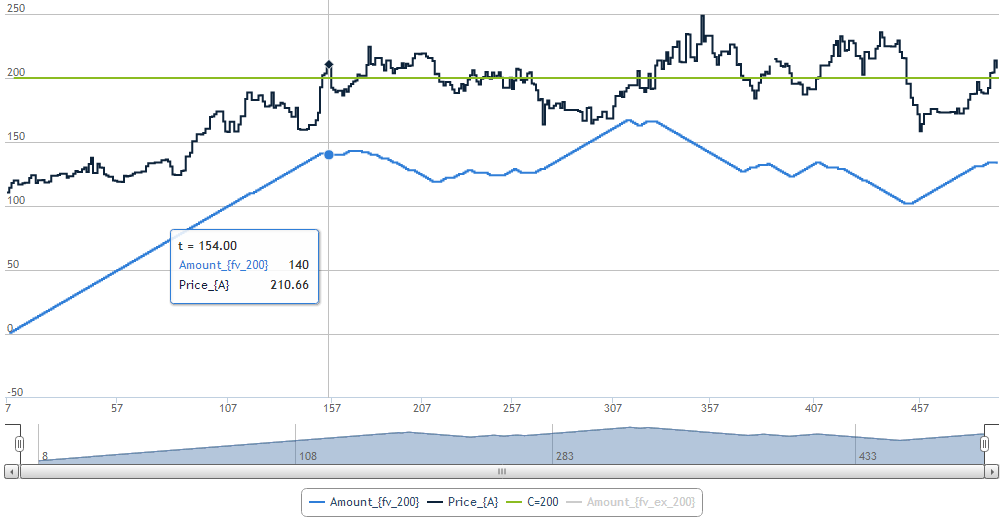
\includegraphics[width=1\linewidth]{fundamentalvalue.png}
\end{figure}
\end{frame}
%------------------------------------------------

\begin{frame}
\frametitle{Mean reversion strategy}
Mean reversion strategy is an instance of a fundamental value strategy with fundamental value equal to some moving average of the asset's price.
\begin{figure}[htbp]
\centering
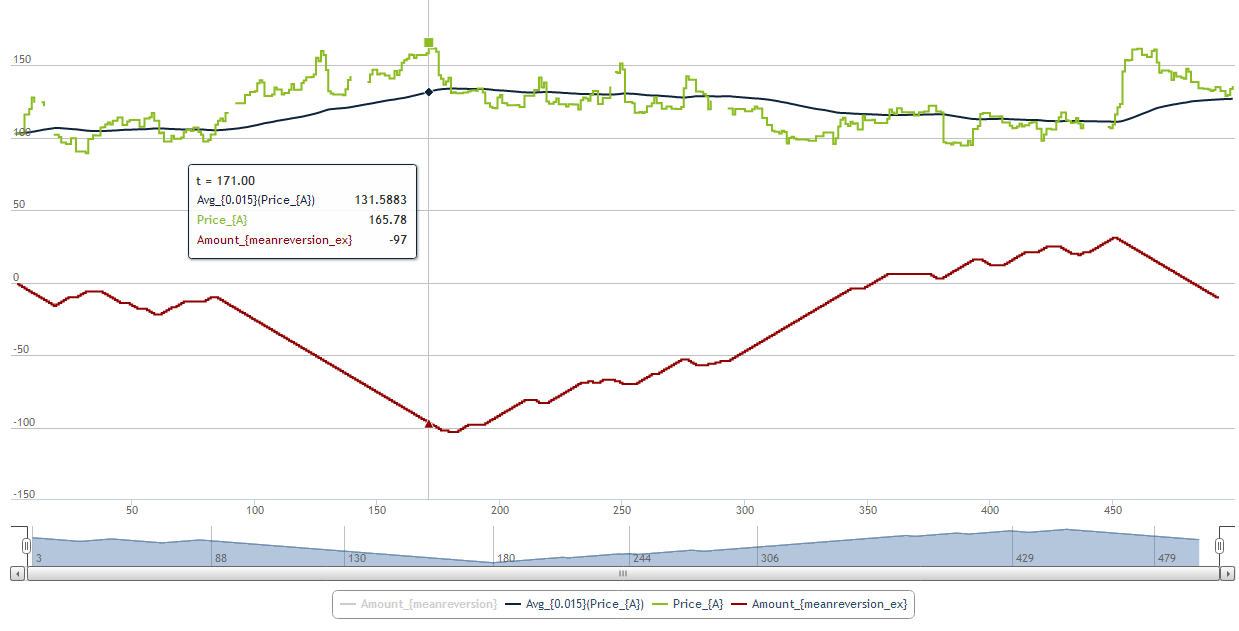
\includegraphics[width=1\linewidth]{meanreversion.png}
\end{figure}
\end{frame}
%------------------------------------------------

\begin{frame}
\frametitle{Liquidity provider}
Liquidity provider sends limit-like orders with a price equal to the current asset's price multiplied by some randomly chosen factor
\begin{figure}[htbp]
\centering
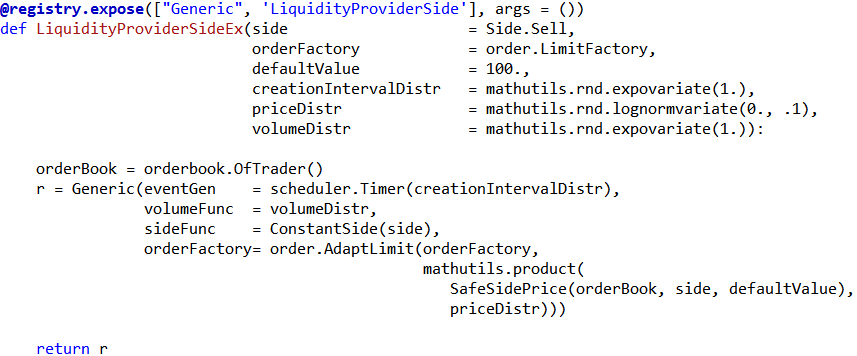
\includegraphics[width=1\linewidth]{liquidityprovider.png}
\end{figure}
\end{frame}
%------------------------------------------------

\begin{frame}
\frametitle{Trade-if-profitable strategy}
Suspends or resumes an underlying strategy basing on its performance backtesting. By default, first derivative of a moving average of 'cleared' trader's balance (trader's balance if its position was cleared) is used to evaluate the efficiency.
\begin{figure}[htbp]
\centering
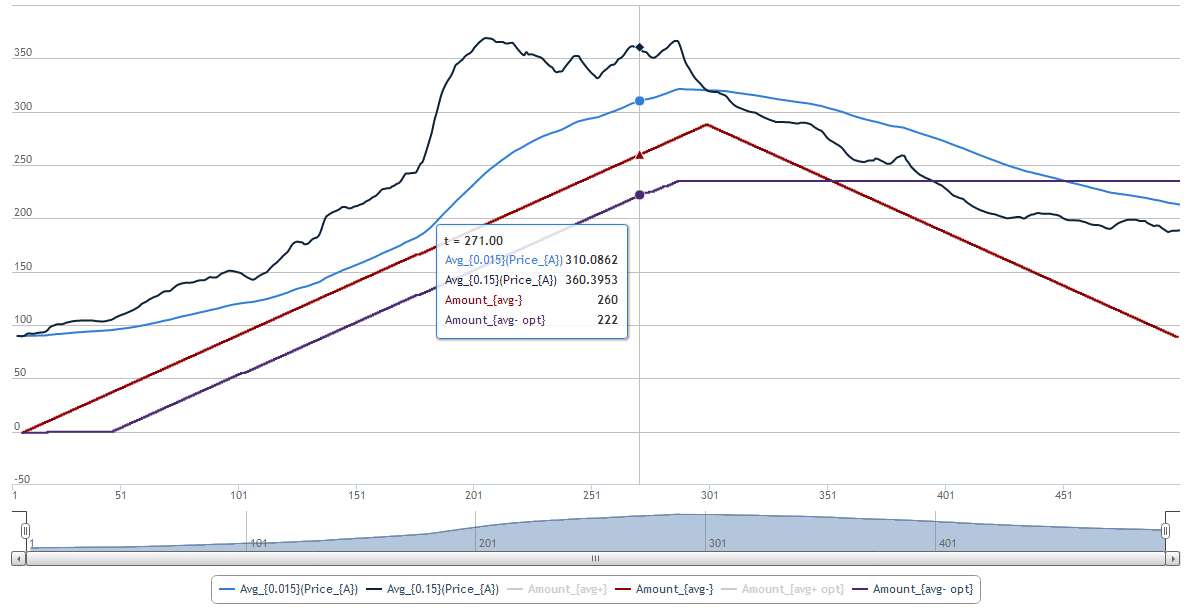
\includegraphics[width=1\linewidth]{tradeifprofitable.png}
\end{figure}
\end{frame}
%------------------------------------------------

\begin{frame}
\frametitle{Choose-the-best strategy}
Backtests aggregated strategies and allows to run only to that one who has the best performance. By default, first derivative of a moving average of 'cleared' trader's balance is used to evaluate the efficiency.
\begin{figure}[htbp]
\centering
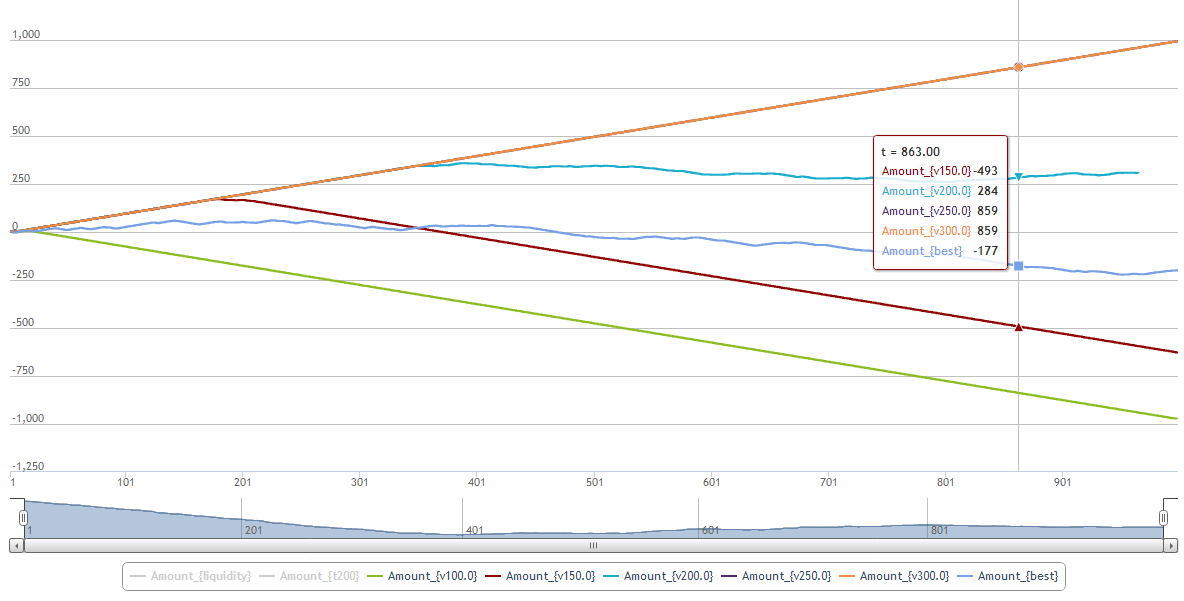
\includegraphics[width=1\linewidth]{choosethebest.png}
\end{figure}
\end{frame}
%------------------------------------------------
\subsection{Observables}
\begin{frame}
\frametitle{Observable}
Traders and order books provide basic accessors to their current state but don't collect any statistics. It order to do it in an interoperable way a notion of observable value was introduced: it allows to read its current value and notifies listeners about its change.
\begin{itemize}
    \item Primitive observables on
    \begin{itemize}
      \item traders: position, balance, market value of the portfolio, 'cleared' balance etc.
      \item order books: ask/mid/bid price, last trade price, price at volume, volume of orders with price better than given etc.
    \end{itemize}
    \item \texttt{OnEveryDt(dt, dataSource)} evaluates \texttt{dataSource} every \texttt{dt} moments of time. Often used with \texttt{Fold(observable, accumulator)} where \texttt{accumulator} may be a moving average or another statistics collector.
\end{itemize}
History of an observable can be stored in a \texttt{TimeSerie} and rendered later on a graph.
\end{frame}
%------------------------------------------------

\section{Using Veusz}
\begin{frame}
\frametitle{Using Veusz}
When developing a new strategy it is reasonable to test it using scripts and visualize results by Veusz
\begin{figure}[htbp]
\centering
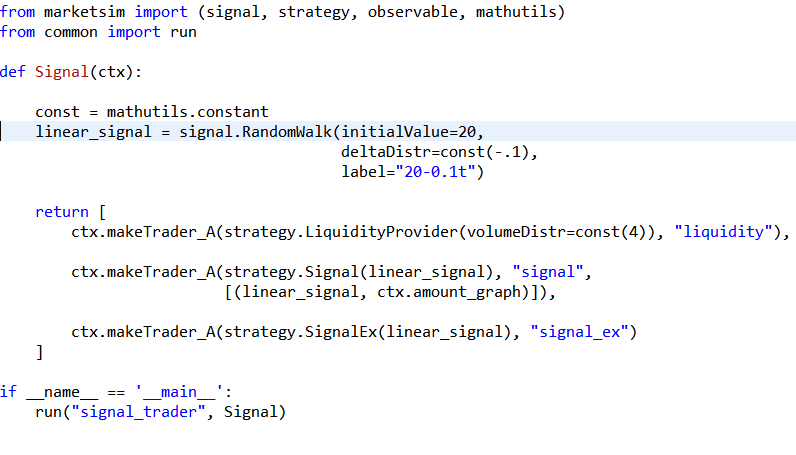
\includegraphics[width=1\linewidth]{using_veusz_code.png}
\end{figure}
\end{frame}

%------------------------------------------------
\begin{frame}
\frametitle{Rendering graphs by Veusz}
\begin{figure}[htbp]
\centering
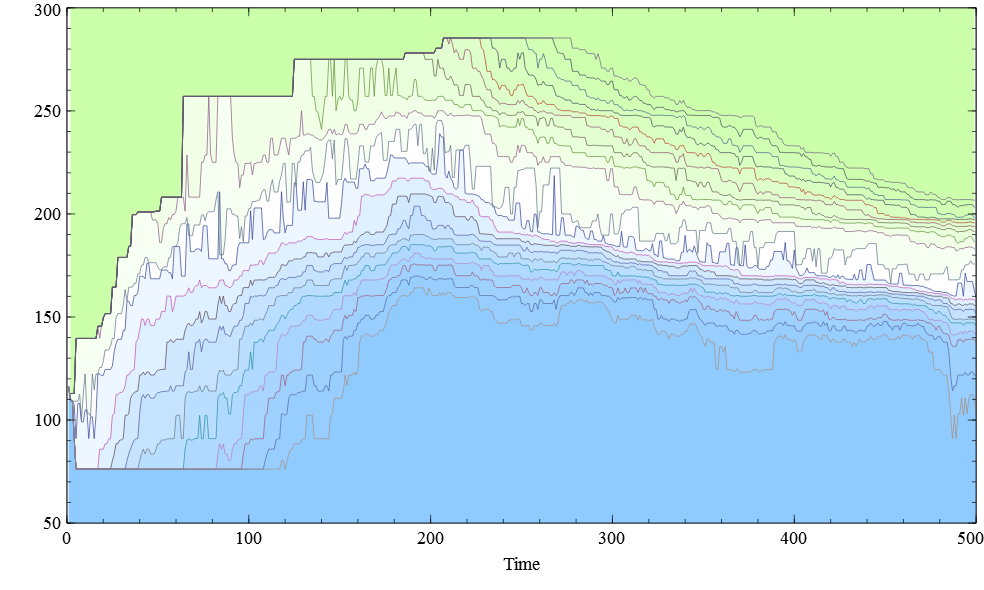
\includegraphics[width=1\linewidth]{veusz_graph.png}
\end{figure}
\end{frame}

%------------------------------------------------

\section{Web interface}
\begin{frame}
\frametitle{Web interface}
Web interface allows to compose a market to simulate from existing objects and set up their parameters
\begin{figure}[htbp]
\centering
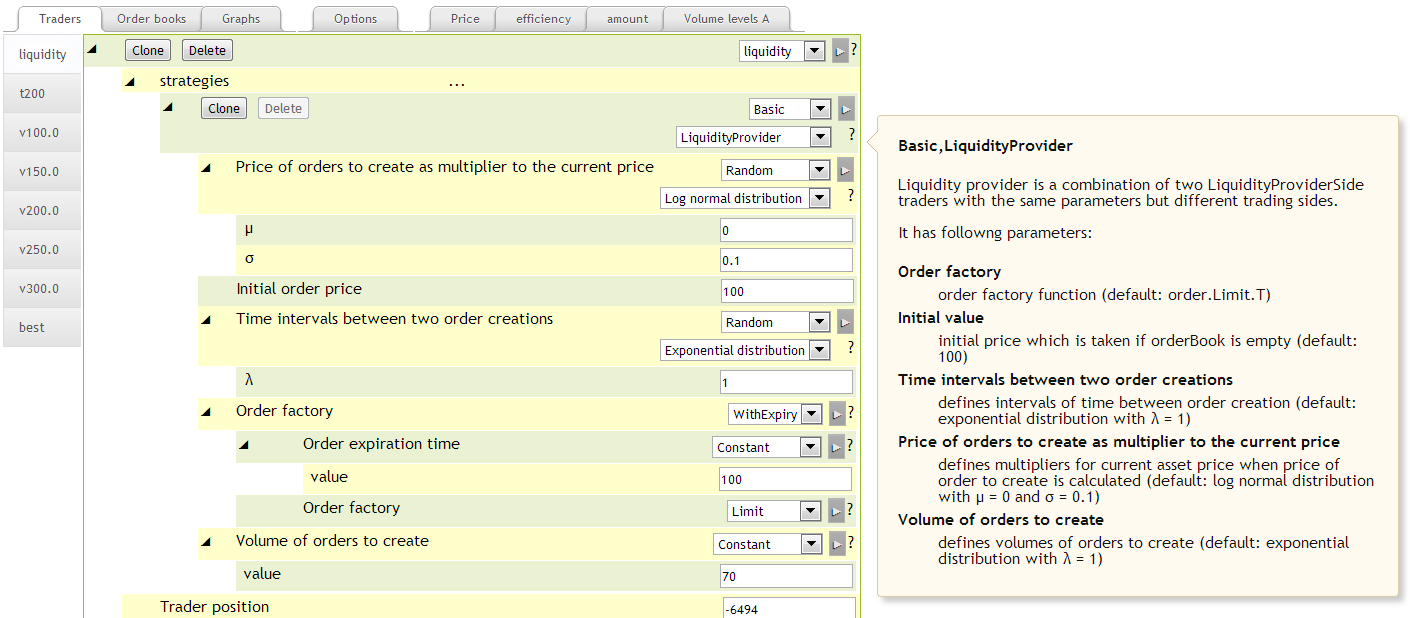
\includegraphics[width=1\linewidth]{js-help.png}
\end{figure}
\end{frame}

\begin{frame}
\frametitle{Time series}
Timeseries field of a trader or an order book instructs what data should be collected and rendered on graphs
\begin{figure}[htbp]
\centering
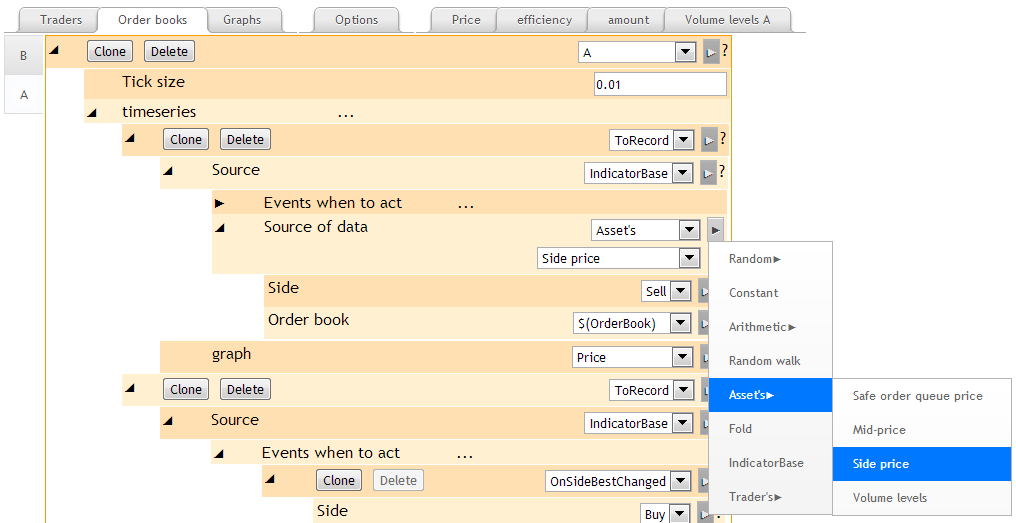
\includegraphics[width=1\linewidth]{js-timeserie.png}
\end{figure}
\end{frame}

\begin{frame}
\frametitle{Rendering results}
\begin{figure}[htbp]
\centering
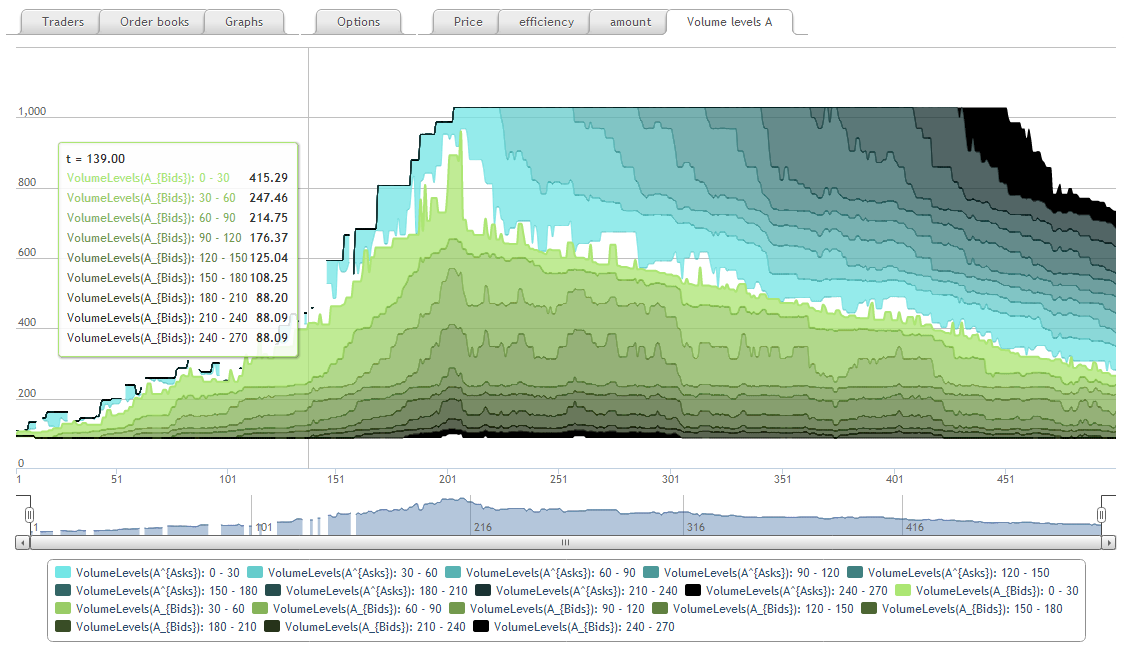
\includegraphics[width=1\linewidth]{js-graph.png}
\end{figure}
\end{frame}

\begin{frame}
\frametitle{Node aliases}
\begin{figure}[htbp]
Object tree nodes can be assigned aliases that can be used later to refer to the sub-tree (explicit by-value or by-reference cloning semantics is to be implemented)
\centering
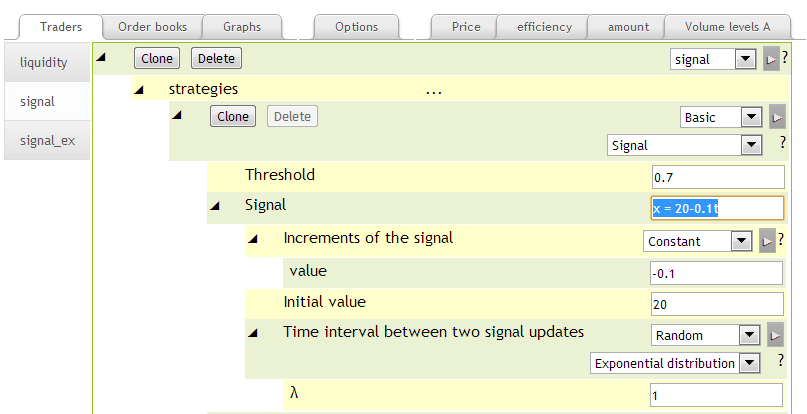
\includegraphics[width=1\linewidth]{js-alias.png}
\end{figure}
\end{frame}

\begin{frame}
\frametitle{Workspaces}
\begin{figure}[htbp]
Every user (identified by browser cookies) may switch between multiple workspaces. Workspaces can be forked, removed or created from a set of predefined ones. 
\centering
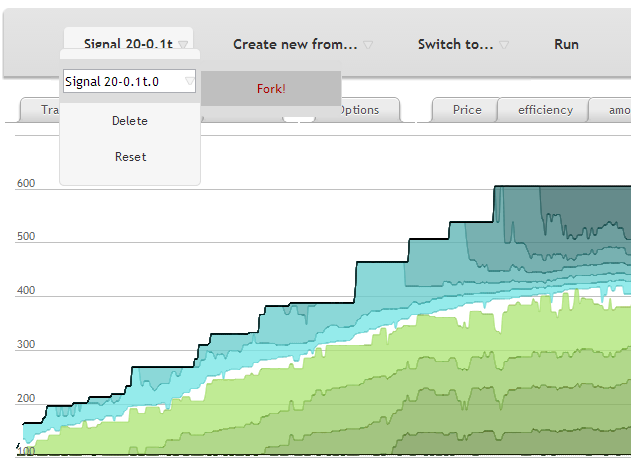
\includegraphics[width=1\linewidth]{js-fork.png}
\end{figure}
\end{frame}

\section{Implementation details}
\begin{frame}
\frametitle{Describing python classes for Web-interface}
\begin{figure}[htbp]
\centering
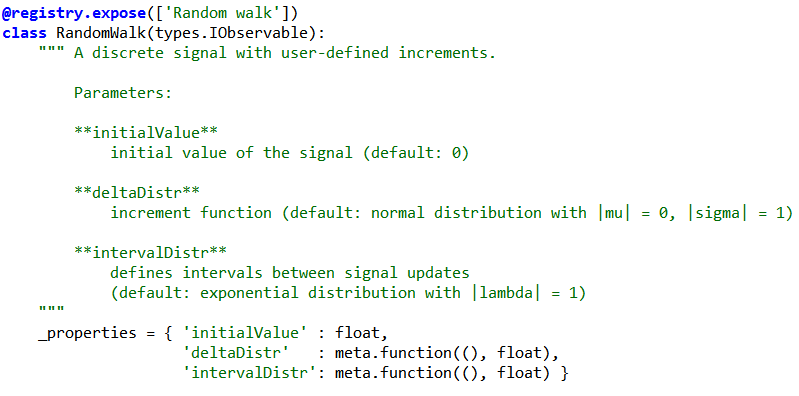
\includegraphics[width=1\linewidth]{metainfo.png}
\end{figure}
\end{frame}


\begin{frame}
\Huge{\centerline{The End}}
\end{frame}

%----------------------------------------------------------------------------------------

\end{document} 